\chapter{Methodology}\label{chap:method}
FL-IDS runs in two phases. \textbf{Phase A} prepares the data, trains the LightGBM classifier, trains the autoencoder over 20 federated rounds with the trust filter, evaluates everything, and saves a model bundle. \textbf{Phase B} loads that bundle, classifies replayed attack traffic on an emulated network and turns the verdict into an OpenFlow rule. Figure~\ref{fig:hld} shows the overall design.

\begin{figure}[H]
\centering
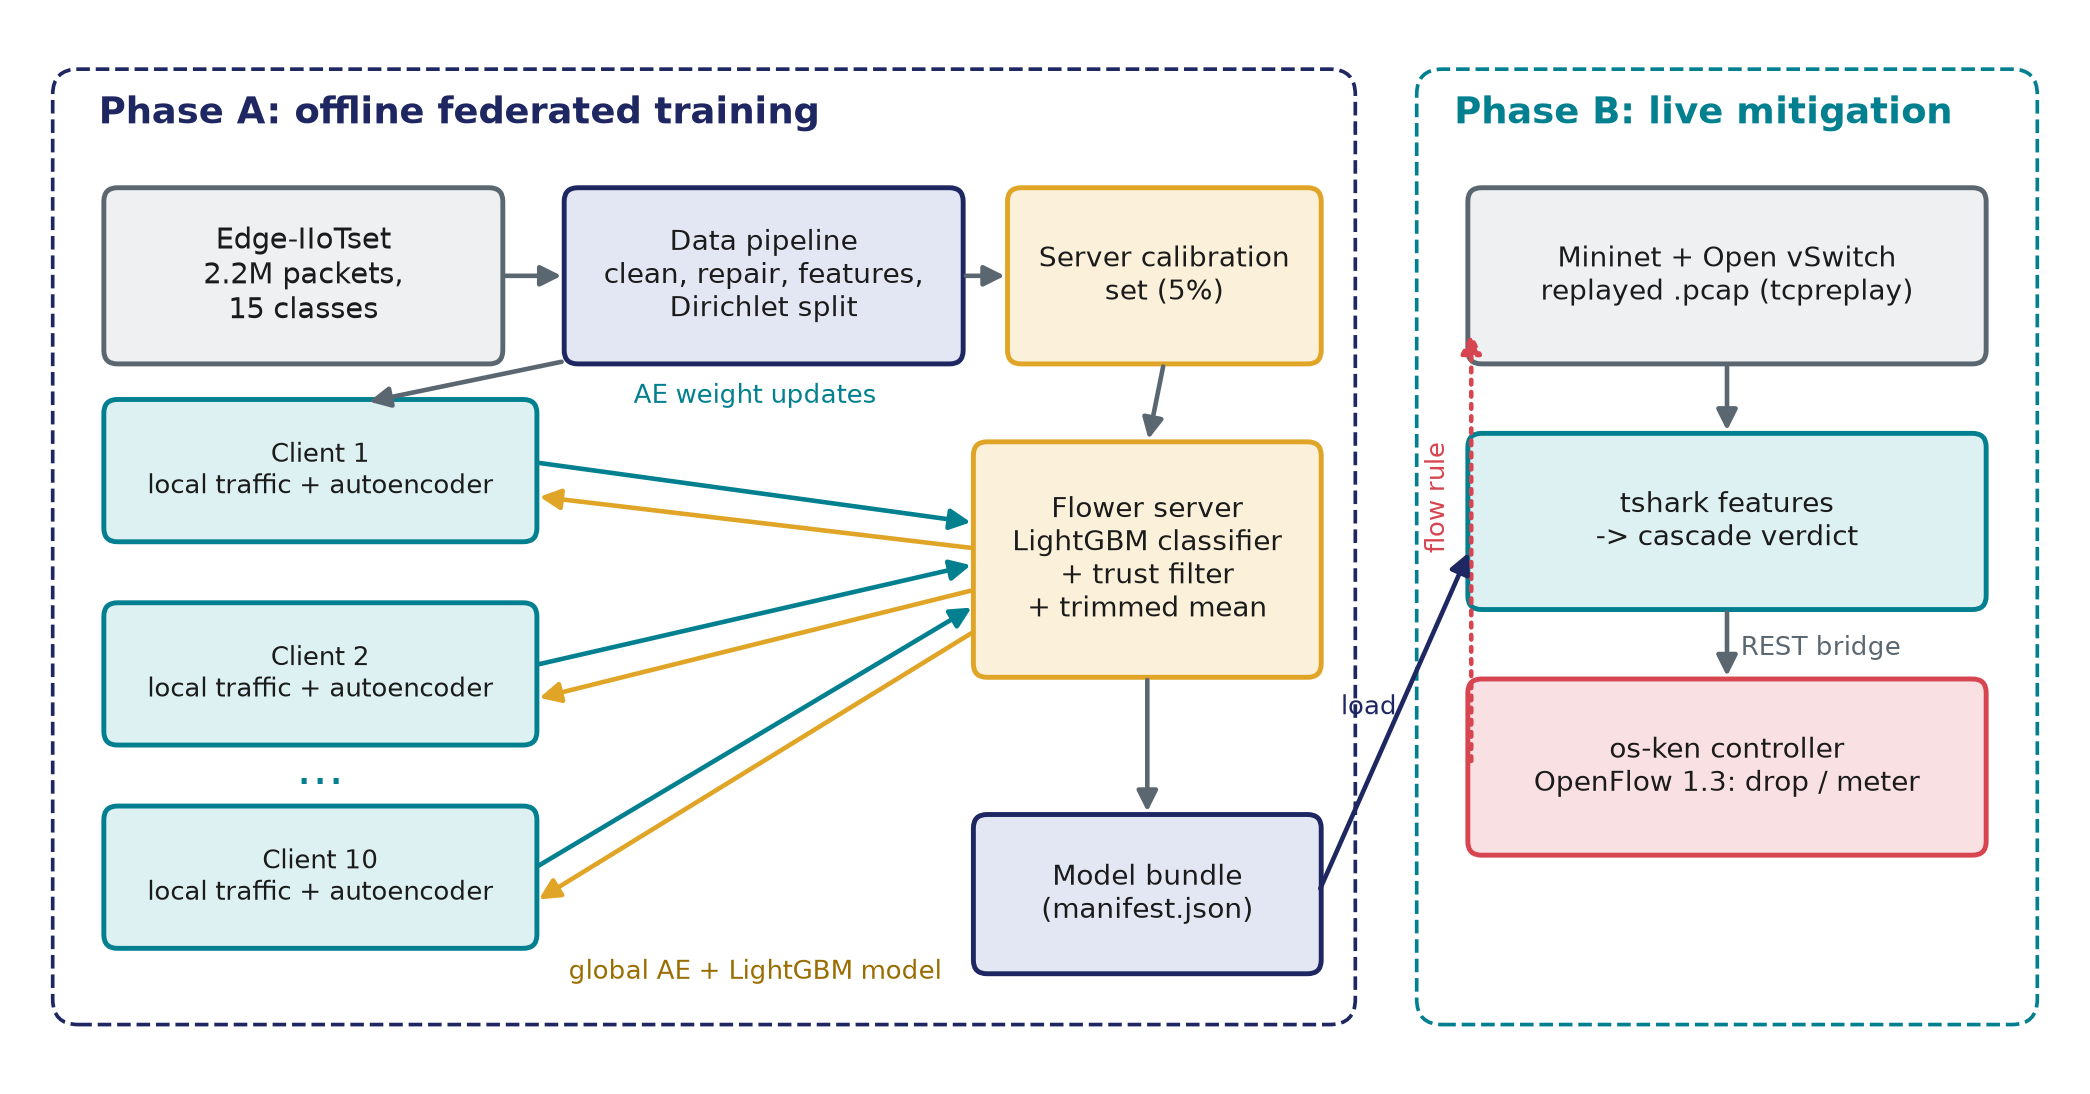
\includegraphics[width=\linewidth]{figures/high_level_design.png}
\caption{High-level design of FL-IDS}
\label{fig:hld}
\end{figure}

\section{Tools and Techniques}
\begin{itemize}
  \item \textbf{LightGBM}~\cite{ke2017lightgbm}: histogram-based gradient-boosted decision trees, used as the first-stage multi-class classifier. Trees work directly on raw feature values, so each client's local normalisation cannot distort the classifier's split thresholds.
  \item \textbf{Autoencoder (PyTorch)}: a dense network $130\rightarrow32\rightarrow16\rightarrow8\rightarrow16\rightarrow32\rightarrow130$ with ReLU activations and a linear output, 9{,}834 parameters in total (7{,}299 with the original 91 features). It learns to reconstruct benign traffic, so a high reconstruction error indicates unusual traffic.
  \item \textbf{Flower}: the federated learning framework. A custom strategy, \texttt{TrustFiltered\-Strategy} (a subclass of FedAvg), implements the trust filter and trimmed-mean aggregation.
  \item \textbf{Cosine similarity, median absolute deviation (MAD) and exponential moving average (EMA)}: the statistics used by the trust filter.
  \item \textbf{Mininet, Open vSwitch, os-ken}: network emulation, the software switch, and the OpenFlow~1.3 controller (os-ken is the maintained fork of Ryu).
  \item \textbf{TShark and tcpreplay}: extracting the dataset's fields from live packets, and replaying captures into the emulated network.
  \item \textbf{Streamlit}: the live dashboard.
\end{itemize}

\section{Data Set With Explanation}
\textbf{Edge-IIoTset}~\cite{ferrag2022edge} was generated on a seven-layer IoT/IIoT testbed (cloud, network functions virtualisation, blockchain, fog, SDN, edge and IoT/IIoT perception layers) with more than ten kinds of sensors, including temperature, humidity, water level, pH, soil moisture, heart rate and flame sensors. They communicate over MQTT and Modbus/TCP. The authors' ML-ready file, \texttt{DNN-EdgeIIoT-dataset.csv}, has 2{,}219{,}201 rows and 63 columns: 61 packet-level fields extracted with tshark, plus \texttt{Attack\_label} and \texttt{Attack\_type}. The 24 per-device and per-attack \texttt{.pcap} captures are also used, for Phase B replay and for repairing corrupted rows.

There are 15 classes: Normal and 14 attacks in five groups. Table~\ref{tab:classes} gives the class sizes after cleaning (current code, before the new features are added).

\begin{table}[H]
\centering
\renewcommand{\arraystretch}{1.15}
\begin{tabular}{|l|l|r|r|}
\hline
\textbf{Group} & \textbf{Class} & \textbf{Rows} & \textbf{\%} \\ \hline
-- & Normal & 1{,}363{,}998 & 71.42 \\ \hline
DoS/DDoS & DDoS\_UDP & 121{,}567 & 6.37 \\
 & DDoS\_ICMP & 67{,}939 & 3.56 \\
 & DDoS\_TCP & 50{,}062 & 2.62 \\
 & DDoS\_HTTP & 48{,}544 & 2.54 \\ \hline
Injection & SQL\_injection & 50{,}826 & 2.66 \\
 & Uploading & 36{,}807 & 1.93 \\
 & XSS & 15{,}066 & 0.79 \\ \hline
Information gathering & Vulnerability\_scanner & 50{,}026 & 2.62 \\
 & Port\_Scanning & 19{,}977 & 1.05 \\
 & Fingerprinting & 853 & 0.04 \\ \hline
Malware & Password & 49{,}933 & 2.61 \\
 & Backdoor & 24{,}026 & 1.26 \\
 & Ransomware & 9{,}689 & 0.51 \\ \hline
Man-in-the-middle & MITM & 406 & 0.02 \\ \hline
\multicolumn{2}{|l|}{\textbf{Total}} & \textbf{1{,}909{,}719} & \\ \hline
\end{tabular}
\caption{Class distribution after cleaning (91 base features)}
\label{tab:classes}
\end{table}

\subsection{Data-quality problems found and fixed}\label{sec:dataquality}
\begin{enumerate}
  \item \textbf{Placeholder label leak.} In the categorical columns, the ``field does not apply'' value is written as \texttt{0} in some source captures and \texttt{0.0} in others, and the spelling follows the label. In \texttt{mqtt.topic}, \texttt{mqtt.conack.flags}, \texttt{mqtt.protoname} and \texttt{dns.qry.name.len}, every Normal row uses \texttt{0} and every attack row \texttt{0.0}. After one-hot encoding, the single column \texttt{mqtt.topic\_0.0} separates benign from attack with an AUROC of 1.0. Both spellings are mapped to \texttt{0} before encoding, after which the strongest single feature has an AUROC of about 0.71. A test guards that no single feature exceeds 0.9.
  \item \textbf{Column-shifted MITM rows.} In the authors' MITM rows, values sit under the wrong column names (for example, their \texttt{tcp.seq} is really \texttt{udp.time\_delta}, with 1.000 agreement). These rows are replaced by re-extracting the authors' own MITM capture with the same field list (1{,}214 rows replaced by 1{,}229).
  \item \textbf{TShark version drift.} Newer tshark prints booleans as \texttt{True}/\texttt{False} and shortens hexadecimal values. Without a fix, this silently zeroed \texttt{tcp.flags.ack} on every live packet in Phase B. Live extraction maps both back to the authors' format.
\end{enumerate}

\subsection{Preprocessing}
Sixteen columns are dropped, following the dataset authors' recipe: identifiers, timestamps, raw payloads and ports, plus \texttt{Attack\_label}, which is fully determined by \texttt{Attack\_type}. Seven nominal columns are one-hot encoded, giving \textbf{91 base features}. Exact duplicate rows are removed (309{,}497 rows), leaving 1{,}909{,}719 rows.

\subsection{New features for the classifier}
Profiling the dropped columns explained why the application-layer attacks were hard to classify. In the SQL\_injection, XSS, Uploading and Password classes, only 5--17\% of packets carry any HTTP content. The rest are content-free TCP handshake and acknowledgement packets to port~80 on the same web server, which look the same whichever attack produced them. Three groups of features were therefore added. IP addresses, absolute time and ephemeral client ports are \emph{never} used as features, because each of them identifies the capture file and hence the label.
\begin{enumerate}
  \item \textbf{Service port (1 feature):} the server side of a connection, $\min(\text{ports} < 32768)$, or $-1$ if there is none (for example ICMP or ARP).
  \item \textbf{Content features (18):} decoded payload length, byte entropy, printable fraction, HTTP request flag, HTTP status code, header count, \texttt{X-} header count, URI length, parameter count, percent-encoding count, file-data length, special-character count, and counts of six generic attack-signature keyword groups (SQL, script/XSS, upload, authentication, traversal/command, scanner tool names).
  \item \textbf{Flow features (20):} packets are grouped into flows by (IP pair, protocol, port pair) in capture order. A new flow starts after a 60\,s idle gap or once a flow has been active for 120\,s, CICFlowMeter's default active timeout~\cite{sharafaldin2018cicids}. Every packet in a flow receives the flow's packet count, duration, packet rate, payload sum/maximum/non-zero share, HTTP request count, maximum status code, SYN, FIN and RST counts, maximum entropy, maximum URI length and keyword totals. IP addresses and times are used only to group packets, never as features.
\end{enumerate}
With all three groups there are 130 features and 1{,}985{,}768 unique rows.

\section{Flow Chart Of Methodology From Start To End}
Figure~\ref{fig:flow} shows the complete sequence of steps, from loading the dataset to verifying the mitigation rule.
\begin{figure}[H]
\centering
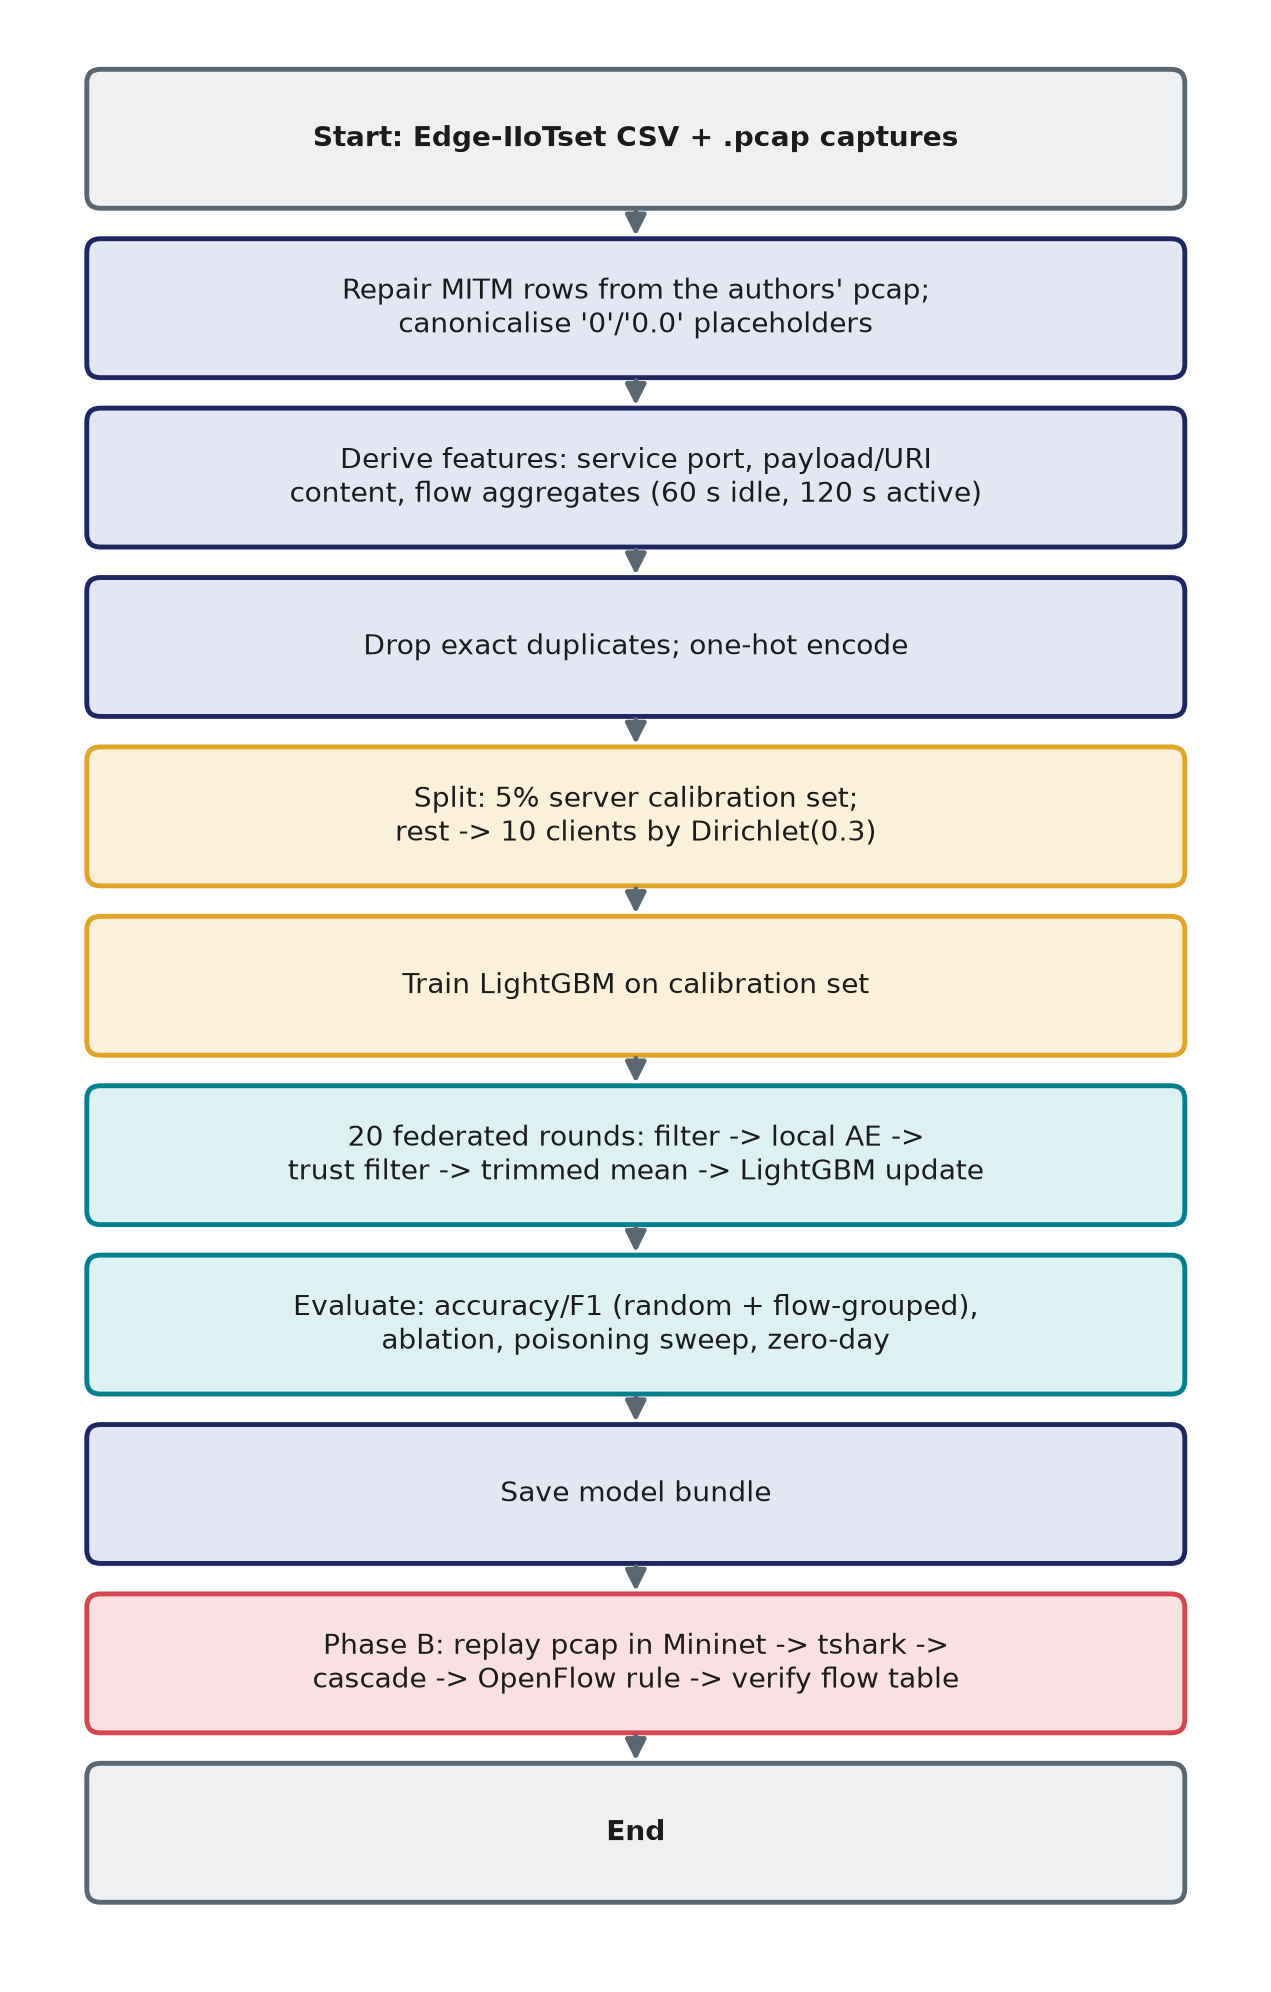
\includegraphics[width=0.62\linewidth]{figures/methodology_flowchart.png}
\caption{Flow chart of the methodology}
\label{fig:flow}
\end{figure}

\section{Explanation Of Methodology In Details With Equations And Formulae}

\subsection{How much data each part uses}
Every packet of the dataset is cleaned and given the new features (2{,}219{,}216 rows, 1{,}985{,}768 unique after de-duplication). How many of them each model trains on differs, and Table~\ref{tab:datascale} lists it. The classifier that meets the accuracy target is trained on most of the data. The federated system uses a smaller share, because its pool is capped at 60{,}000 rows to keep the roughly 150 evaluation runs practical.
\begin{table}[H]
\centering
\small
\renewcommand{\arraystretch}{1.2}
\begin{tabular}{|>{\raggedright\arraybackslash}p{4.4cm}|>{\raggedright\arraybackslash}p{4.7cm}|>{\raggedright\arraybackslash}p{4.7cm}|}
\hline
\textbf{Part} & \textbf{Trained on} & \textbf{Evaluated on} \\ \hline
Final classifier (accuracy target) & 1{,}429{,}825 rows (72\%), plus 158{,}870 for early stopping (8\%) & 397{,}073 unseen rows (20\%); whole connections held out \\ \hline
Same classifier, 5\% share only & 89{,}359 rows, plus 9{,}929 for early stopping & the same 397{,}073 rows \\ \hline
Federated: server bootstrap classifier & 79{,}430 rows (calibration set) & 19{,}858 rows held back \\ \hline
Federated: client autoencoders & 45{,}474 rows across 10 clients (736 to 11{,}549 each), plus 5{,}530 benign rows for thresholds & 8{,}996 client test rows \\ \hline
\end{tabular}
\caption{Training and evaluation rows for each part (130 features, seed 42)}
\label{tab:datascale}
\end{table}
The 5\%-only row shows that the federated bootstrap loses little from its smaller training set: 99.7\% accuracy and 0.979 macro F1 on the same 397{,}073 test rows, against 0.983 for the full classifier.

\subsection{Non-IID partition and per-client normalisation}
A stratified 5\% of the rows is held on the server as the calibration set. The remaining federated pool (subsampled to 60{,}000 rows to keep the roughly 150 evaluation runs practical) is split across $N=10$ clients. For each class $k$ a proportion vector is drawn,
\begin{equation}
  \mathbf{p}_k \sim \mathrm{Dir}(\alpha\mathbf{1}_N), \qquad \alpha = 0.3,
\end{equation}
and the class's rows are divided in those proportions~\cite{hsu2019noniid}. Smaller $\alpha$ gives more skew. Each client keeps 15\% as a test slice and 15\% of its benign remainder as a benign validation slice. For the autoencoder only, client $i$ standardises features with its own training mean $\mu_i$ and standard deviation $\sigma_i$, clipped at $\pm10$:
\begin{equation}
  \tilde{x} = \mathrm{clip}\!\left(\frac{x-\mu_i}{\sigma_i},\,-10,\,10\right).
\end{equation}
The clip is needed because a counter feature can barely vary inside one skewed shard. Without it, one client's benign validation loss stayed near 400 for 20 rounds; with it, the loss fell to 0.0146.

\subsection{Stage 1: LightGBM classifier}
LightGBM builds an additive model of $T$ trees per class, $F_k(\mathbf{x}) = \sum_{t=1}^{T} f_{t,k}(\mathbf{x})$, with class probabilities
\begin{equation}
  P(y=k\mid\mathbf{x}) = \frac{e^{F_k(\mathbf{x})}}{\sum_{j=1}^{15} e^{F_j(\mathbf{x})}},
\end{equation}
trained by minimising the weighted multi-class log loss
\begin{equation}
  \mathcal{L} = -\frac{1}{\sum_n w_n}\sum_{n} w_{n}\,\log P(y=y_n\mid\mathbf{x}_n) + \lambda_2 \sum_{t}\lVert \mathbf{v}_t\rVert^2 ,
\end{equation}
where $\mathbf{v}_t$ are leaf values and $\lambda_2 = 1$. The sample weight $w_n$ is a square-root inverse class frequency, recomputed for every training set (the bootstrap and each incremental update),
\begin{equation}
  w_n = \sqrt{\frac{\max_j N_j}{N_{y_n}}},
\end{equation}
so a rare class such as Fingerprinting counts more without being blown up the way full inverse-frequency weights would. In the federated pipeline the classifier uses 300 rounds, learning rate 0.05 and 31 leaves, trained deterministically on one thread so runs are reproducible. The stand-alone accuracy experiments of Section~5.1 used 63 leaves, learning rate 0.1, feature and bagging fractions of 0.8, and early stopping after 50 rounds without improvement on a 10\% validation split.

\subsection{Stage 2: autoencoder and threshold}
Each client trains the autoencoder $g_\theta$ on the rows the current classifier passes (predicted Normal, or an attack with probability below 0.7). It minimises the mean squared reconstruction error
\begin{equation}
  e(\mathbf{x}) = \frac{1}{d}\sum_{j=1}^{d}\big(\tilde{x}_j - g_\theta(\tilde{\mathbf{x}})_j\big)^2
\end{equation}
with Adam (learning rate $10^{-3}$, 5 local epochs, batch size 64). The client's threshold is recomputed every round as the 97th percentile of $e$ on its benign validation slice, $\tau_i = Q_{0.97}\{e(\mathbf{x}) : \mathbf{x}\in V_i\}$.

\subsection{Cascade decision rule}
Figure~\ref{fig:cascade} shows the shared decision rule. With $\hat{k}=\arg\max_k P(k\mid\mathbf{x})$ and $p = P(\hat{k}\mid\mathbf{x})$:
\begin{equation}
\text{label}(\mathbf{x}) =
\begin{cases}
  \hat{k} & \text{if } \hat{k}\neq\text{Normal and } p \geq 0.7,\\
  \text{anomalous} & \text{else if } e(\mathbf{x}) > \tau_i,\\
  \text{benign} & \text{otherwise,}
\end{cases}
\end{equation}
with confidence $p$ for a known attack and $\mathrm{clip}(e/\tau_i - 1,\,0,\,1)$ for an anomaly.
\begin{figure}[H]
\centering
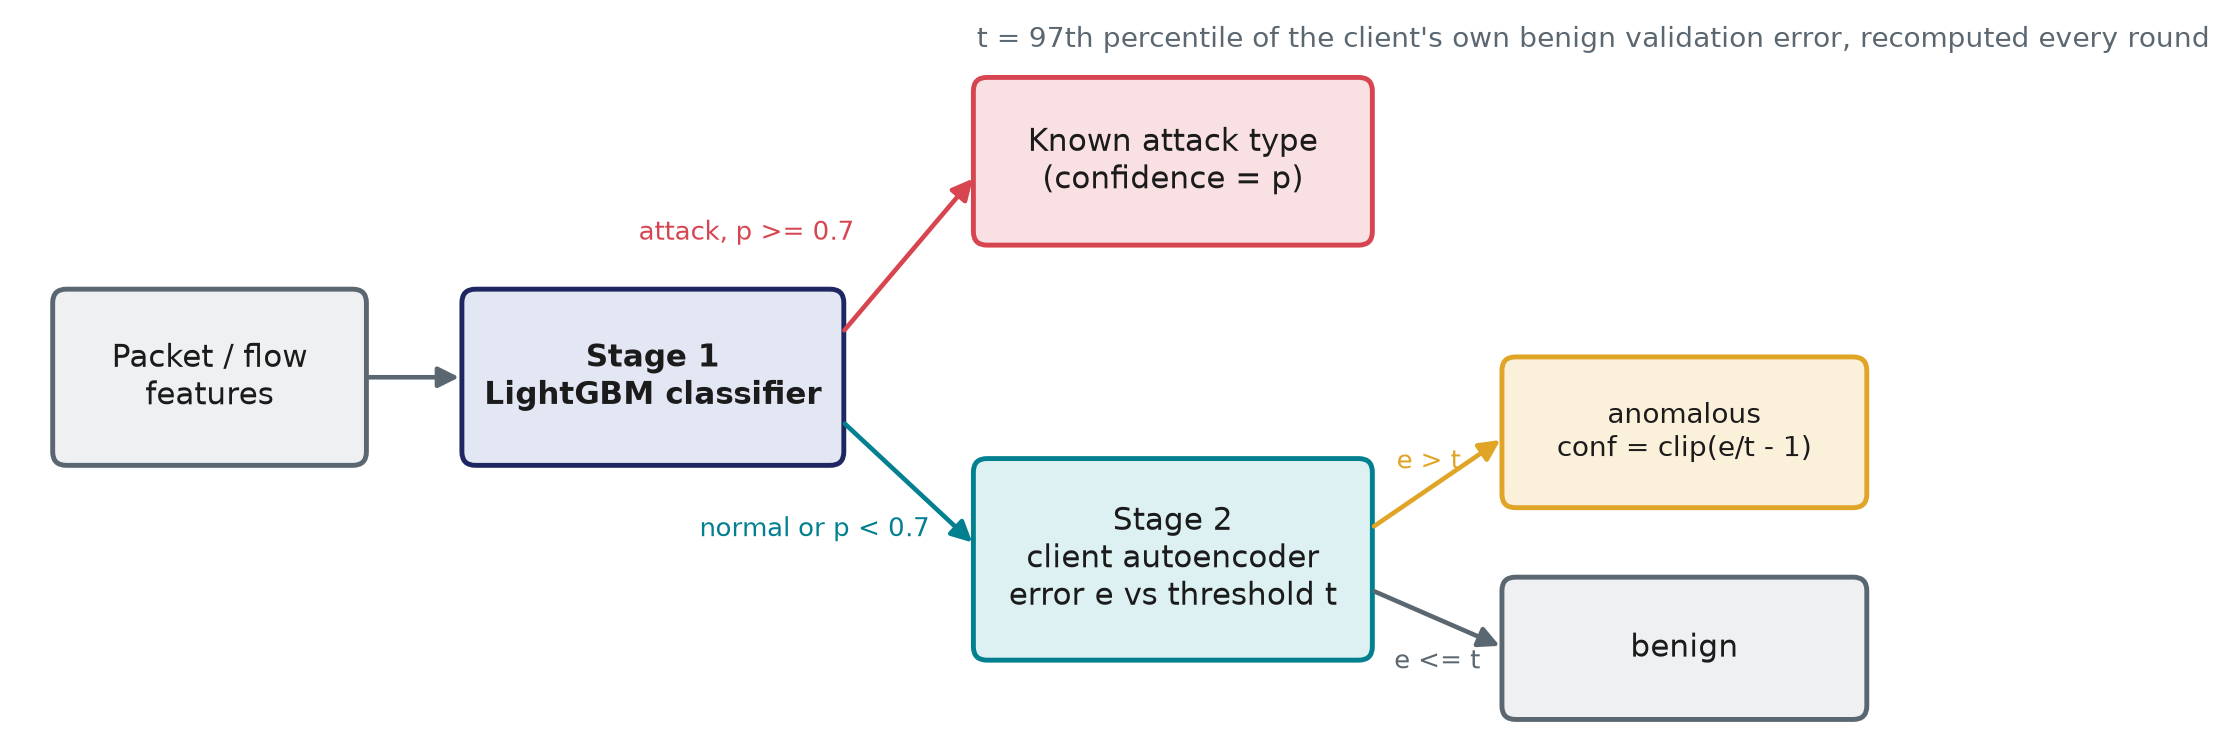
\includegraphics[width=0.92\linewidth]{figures/cascade_rule.png}
\caption{Two-stage cascade decision rule}
\label{fig:cascade}
\end{figure}

\subsection{Trust filter and robust aggregation}
Let $\mathbf{w}^{(r)}$ be the global weights at the start of round $r$ and $\mathbf{w}_i$ client $i$'s weights after local training. The filter works on \emph{deltas} $\Delta_i = \mathbf{w}_i - \mathbf{w}^{(r)}$. The reference direction is the coordinate-wise median $\mathbf{m} = \mathrm{median}_i(\Delta_i)$, and each client's similarity is
\begin{equation}
  s_i = \frac{\Delta_i\cdot\mathbf{m}}{\lVert\Delta_i\rVert\,\lVert\mathbf{m}\rVert}.
\end{equation}
Trust is a running average, starting at $T_i=1$:
\begin{equation}
  T_i \leftarrow (1-\beta)\,T_i + \beta\,\frac{s_i+1}{2}, \qquad \beta = 0.3 .
\end{equation}
Client $i$ is excluded in round $r$ if any of these holds:
\begin{equation}
  s_i < \tilde{s} - 3\,\mathrm{MAD}(s) \quad\text{or}\quad s_i < 0 \quad\text{or}\quad T_i < 0.5 ,
\end{equation}
where $\tilde{s}$ is the median similarity. Surviving deltas are clipped to twice the median norm $\nu$,
\begin{equation}
  \Delta_i' = \Delta_i\cdot\min\!\left(1,\ \frac{2\nu}{\lVert\Delta_i\rVert}\right),
\end{equation}
and combined coordinate-wise with a 15\% trimmed mean, which drops the largest and smallest $\lfloor0.15\,n\rfloor$ values in each coordinate:
\begin{equation}
  \mathbf{w}^{(r+1)} = \mathbf{w}^{(r)} + \mathrm{TrimMean}_{0.15}\big(\{\Delta_i'\}\big).
\end{equation}
The test attacker trains honestly and then sends $-5\Delta_i$ (sign flip, amplified five times), while claiming the largest client's example count. Figure~\ref{fig:round} summarises one round.
\begin{figure}[H]
\centering
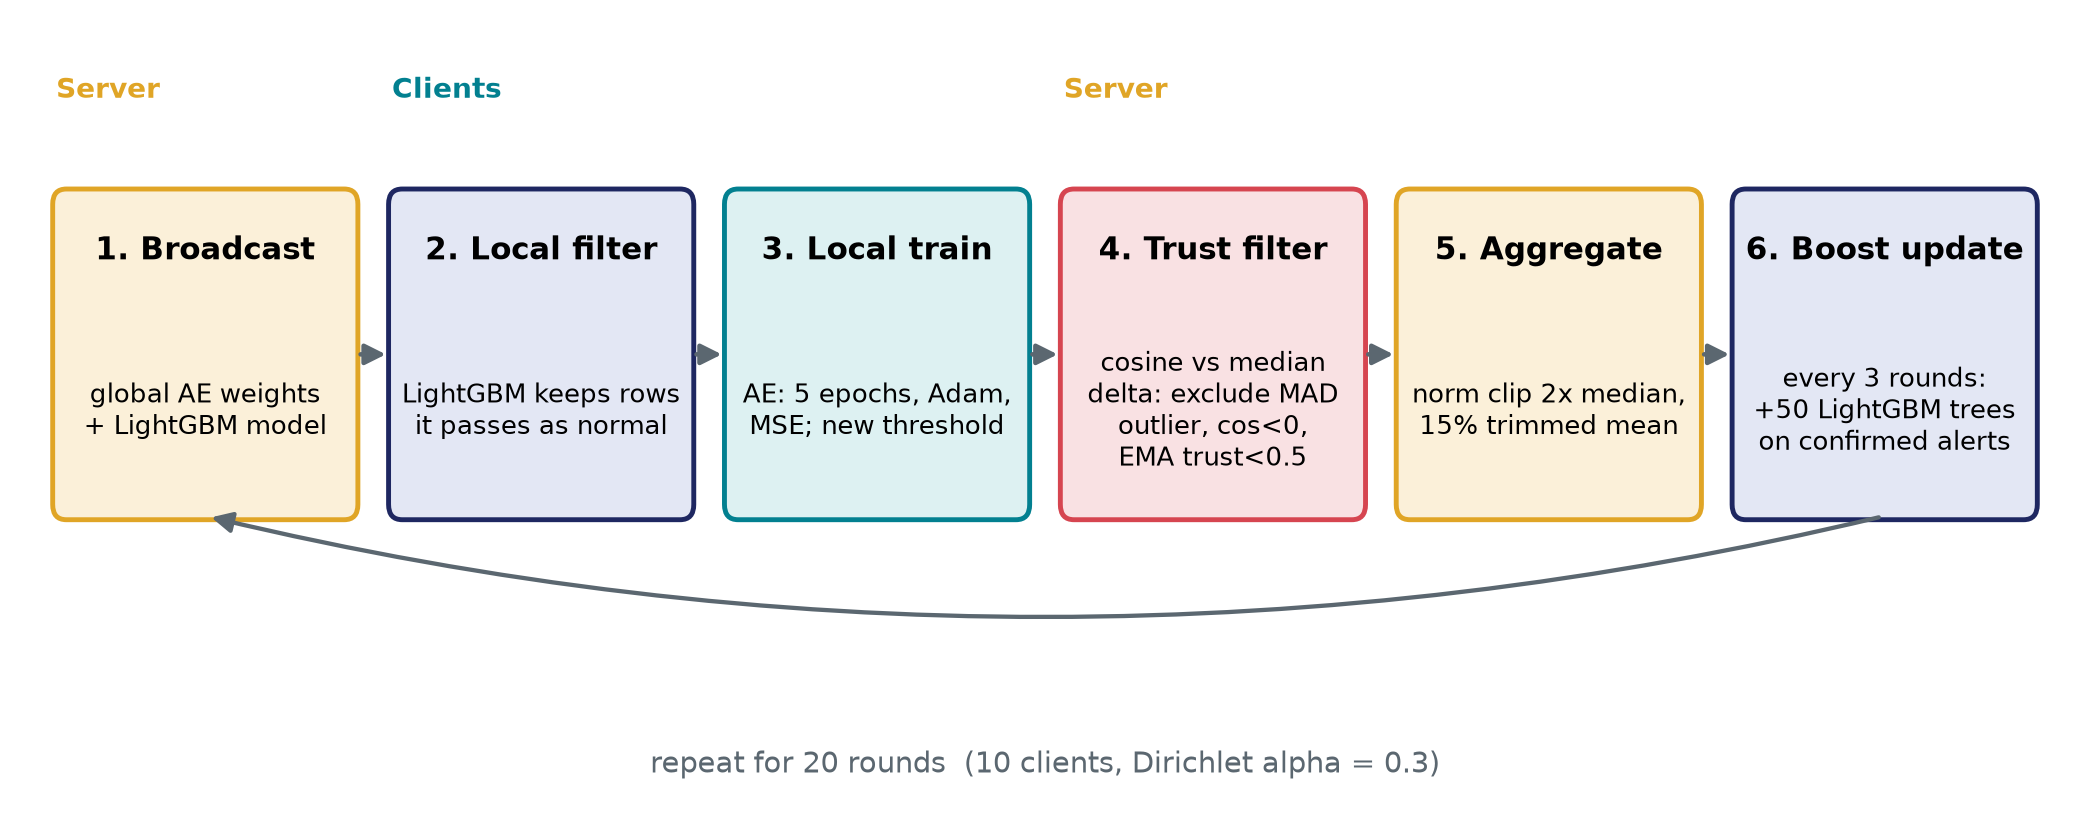
\includegraphics[width=\linewidth]{figures/fl_round.png}
\caption{One federated round}
\label{fig:round}
\end{figure}

\subsection{Incremental classifier update}
Every 3 rounds, each client that survived the filter surfaces up to 50 rows its autoencoder flagged, with analyst-confirmed labels. The server continues training LightGBM with 50 more trees on the calibration set plus all collected alerts, or retrains from scratch if the alerts contain a class the model has never seen. This relaxes the ``no raw traffic leaves a client'' rule for these capped, confirmed alerts only, and is reported as a privacy trade-off.

\subsection{SDN mitigation}
In Phase B, Mininet creates one host per federated client on one Open vSwitch switch, controlled by os-ken over OpenFlow~1.3. A real attack capture is replayed with tcpreplay. TShark extracts all 61 of the dataset's fields, the service-port, content and flow features are derived from the capture with the same code as in training, each row is scored with that host's own scaler and threshold, and the most frequent non-benign label becomes the device verdict. A Flask bridge maps the verdict to an action: \emph{block} (a drop rule on the source IP) if confidence $\geq0.85$, \emph{rate-limit} (an OpenFlow meter) if $\geq0.5$, otherwise allow. The installed rule is then read back from the switch's flow table to confirm it.

\subsection{Evaluation metrics}
With $TP_k$, $FP_k$, $FN_k$ counted per class $k$ over $K$ classes:
\begin{align}
  \text{Accuracy} &= \frac{\#\text{correct}}{\#\text{test rows}}, &
  P_k &= \frac{TP_k}{TP_k+FP_k}, &
  R_k &= \frac{TP_k}{TP_k+FN_k},\\
  F1_k &= \frac{2P_kR_k}{P_k+R_k}, &
  \text{Macro F1} &= \frac{1}{K}\sum_{k}F1_k .
\end{align}
Because 71\% of traffic is benign, accuracy alone hides poor results on rare attacks, so macro F1 is reported next to it. A class with no rows in a test split (MITM is a single flow) is left out of that split's macro average. Two splits are used: a \textbf{stratified random 80/20 split} of rows, and a stricter \textbf{flow-grouped 80/20 split} (stratified group k-fold), in which every flow lies entirely in training or entirely in test, so the model cannot score well by memorising connections. The \textbf{ambiguity ceiling}, the accuracy of an oracle that gives every distinct feature vector its majority label, shows how separable the classes are with a given feature set. For the federated system, attack macro-recall, benign false-positive rate, zero-day macro-recall (leave one attack class out of all training data, then score it) and malicious-client survival rate are also reported.
